\documentclass[hidelinks,english]{article}

\usepackage{graphicx}
\usepackage{grffile}
\usepackage[T1]{fontenc}
\usepackage{babel}
\usepackage{wrapfig}
\usepackage{hyperref}

\date{\today}

\graphicspath{{Pictures/}}
\begin{document}	
	\begin{titlepage}
		\pagenumbering{gobble}
		\begin{figure}[!t]
			
\includegraphics[width=\linewidth]{up_logo.png}
		\end{figure}
		\vspace*{\stretch{1.0}}
		\begin{center}
			\huge{Software Requirements Specification and Technology Neutral Process Design\\}
			\huge{Mindmap PIM}\\
			\large{Client: IMINISYS}\\
			\vspace{10mm}
			\huge{Team: A-Cube-N}\\
		\end{center}
		\begin{center}
			\begin{tabular}{ c c c }
				Dunkley, Nathan & Grobler, Arno & Lochner, Amy \\
				\texttt{14145759} & \texttt{14011396} & \texttt{14038600}\\
				& Maree, Armand &\\
				& \texttt{12017800} &
			\end{tabular}
		\end{center}
		\begin{center}
			Department of Computer Science, University of Pretoria
		\end{center}
		\vspace*{\stretch{2.0}}
	\end{titlepage}
	\newpage
	\tableofcontents
	\newpage
	\pagenumbering{arabic}
	
	\section{Introduction} 
		\paragraph\indent
		People of this day and age often make use of many technologies and platforms for the purpose of staying in contact with people, sharing moments with friends, communicating with people and organising their day-to-day lives. Generally all the above tasks of a person in the 21st century are done on different platforms for example Facebook, Email and Google Calendar. This project serves to provide the people described above, with a single Personal Information Manager (PIM) platform with which they can interact to make use of the functionality from other platforms. A PIM as defined by \textit{TechTerms} is "a software application that serves as a planner, notebook, and address book all in one. It can also include things like a calculator, clock , and photo album." 
	
	
	\section{Vision}
		\paragraph\indent
		The vision of this project is to create a PIM which extracts data from various existing platforms such as Facebook, Gmail, Google Calendar etc. The application will make use of various means to extract data, determine the general topic of the data then either construct a new branch in the mind map or add the data as a sub branch in the diagram. The hope is that this will simplify the users life by only needing one application to 'monitor' all other platforms on which they might have an account and manage the information of those platforms from our application. The mind map will work in a similar fashion as our minds work. Where the exploration of one topic may lead to the exploration of another topic that is related to the user specifically. Hence the "mind" map, it is a map of your mind visualized by the topics that come up in your life.
	
	\section{Background}
		\paragraph\indent
		We got elected for this project by including it as one of our top 3 choices for the projects that we wanted to do most. Once this project was elected for us to do, we began to learn more about what the client expected from us..

		\subsection{Future business/research opportunities}
			\paragraph\indent
			The Mind Mapped PIM project provides an opportunity for us to create something that helps to simplify the user's life. It will do this by organizing all relevant information into one system. It can also help the user to plan out their daily and weekly schedules which can lead to reduced stress on the user.
		
		\subsection{The Client's Problem}
			\paragraph\indent
			The client wants to have a way of displaying all relevant information in one place in the form of a mind map. This will help to organize general life events such as meetings and current tasks that need to be completed. This information will come from different sources and enables the user to see all relevant information without having to go to each source individually
		
	\section{Important Terminology}
		\begin{itemize}
			\item \textbf{MyBubbles} A potential commercial name for the application.
			\item \textbf{Bubble} A single node in the mind map.
			\item \textbf{Bubble Map} The mind map that is presented to the user.
			\item \textbf{PIM} Personal Information Manager such as Google Calendar and social media platforms like Facebook.
		\end{itemize}	
	
	\section{Architecture Requirements}
		\subsection{Access Channel Requirements}
    		\subsubsection{Human Access Channels}
    			\paragraph\indent
                Users  will access the "Mind mapped PIM" system through a website. It should be available to anyone wishing to sign up  through any browser i.e. Chrome, Mozilla Firefox, Internet Explorer, Safari and Edge. When on the website, the user will have to log in, the option given to log in with their Facebook or Google user name and passwords.  The website will be under strict standards-compliance that is having the website comply with the World Wide Web Consortium (W3C) (W3C, 2016)  so that the website will run on every browser exactly the same. The website should be mobile friendly as to be able to scale down to a phone screen size and still be usable and interactive. Offline capabilities for users who have already used the service before should also be allowed.
            \subsubsection{System Access Channels}
            	\paragraph\indent
                RESTful web services will as the system access channel for its lightweightedness, maintainability, and scalability. It will use URI's to allow easy access from the client side web service to server side. 
		
		\subsection{Quality Requirements}
			\paragraph\indent
            The following quality requirements have been placed in order of priority.
            \subsubsection{Performance}
            	\paragraph\indent
                Performance has the highest priority since this system has to be real time. Any new information that is updated on the respective websites and email clients should, in the least amount of time possible, update the mind map too.
                
                \paragraph\indent
                Performance in terms of front-end should also be addressed. The system is a fully graphic website and thus should give the user the most fluid and smooth experience. To implement a fast interactive system technologies such as SVG or HTML canvas can be used to render the graph with smooth user interaction.
            \subsubsection{Usability}
            	\paragraph\indent
                Usability is the second highest priority as the system is fully graphic in terms of what the end user will use. The system needs to have a very good UX and must be completely user friendly so it is not difficult to use. The end goal is to let the system give benefit to it being graphic so the user can interpolate the data, and not make it more difficult
            \subsubsection{Reliability}
            	\paragraph\indent
                The system needs to be reliable, since it has to provide information in real time. this cannot happen if the system is constantly down or can only cater for X amount of users before it starts slowing down. When, for example, a user clicks to expand a bubble the result should be almost instant and not break the graph or slow down the whole system because it is retrieving a few bubbles.
                
                \paragraph\indent
                Reliability also refers to providing accuracy, and such needs to be implemented to provide the correct information to the right bubbles.
                
                \paragraph\indent
                Implementation of reliability should be done in two parts, namely first prevention of faults, and secondly detection of faults.
            \subsubsection{Scalability}
                this system needs to be highly scalable both in terms in the non restriction on the amount of users that can use the system simultaneously and the amount of data stored of each user that needs to be both stored and displayed without hindering the rest of the system.
                
                \paragraph\indent
                The amount of users using the system could be large at any time, and the use of the system by one user should not impact the use of the system by another user. The actual Mind map should also not become slower or unresponsive if the amount of bubbles grow, which it will.
                
                \paragraph\indent
                Polling of the respective social media and email should also be considered. The increase in the amount of threads used for this operation should not make the system unresponsive
            \subsubsection{Flexibility}
            	\paragraph\indent
                The system must be flexible in terms of plugablity of subsystems that are used namely our social media and emails. Since all of these system are different and use different API's and architectures. The system should be able to handle this, and any future systems that need to be added.
                
                \paragraph\indent
                Some users will not have a Facebook account for example, and thus the system should still irrespective if the user has a certain social media.

            \subsubsection{Security}
            	\paragraph\indent
                The system should be very secure since it is using private information that belongs solely to that user. Private information such as emails and photos isn't something that users would like other people seeing. Thus implementation of a secure log in process has to be implemented. Since Google and Facebook have both good log in systems, we will use that to log in to the system.\\
                If a user prefers to not have certain features of social media, such as only look at posts and photos on Facebook but not post on their behalf, then the system should cater for that.
            \subsubsection{Auditability/Monitorability}
            	\paragraph\indent
                Logs of all actions and settings of the user should be maintained. When the user logs back in at a different time, the graph that was displayed before should be displayed again and updated with new things that had happened while the user was offline. Settings should remain the same between sessions.
            \subsubsection{Integrability}
            	\paragraph\indent
                The system should be integrable in terms of how well it integrates with other systems like Facebook and Google. This information should be easy to access and does not affect the functioning of the overall system.

		
		\subsection{Integration Requirements}
			\begin{enumerate}
		        \item \textbf{HTTP:}\\
		            This is the main protocol for all websites and will be the interface for the user to easily navigate the system.
		        \item \textbf{SMTP and IMAP:}\\
		            Sometimes a user does not want to connect their social media for safety concerns and so the system cannot use the APIs required and thus will need to manually get the information by making use of IMAP to retrieve and sort though the users mailbox and SMPT to still have the option for the system to send emails on behalf of the user. This allows the system to still have functionality without any specified API's for those users who do not wish to share that information or who do not own social media.
		        \item \textbf{REST:}\\
		            As mentioned before, REST will be implemented. It is simple to implement and integrates well with systems already operational. REST integrates will with HTTP and follows a client-server model which is something our system utilizes. REST is vital to the use of API's to gain access to information of social media of the user.
		        \item \textbf{TCP:}\\
		            This protocol will be needed to establish network connections between the users computers and the system servers. Theses data streams can then be exchanged between the connected hosts. TCP will allow for error detection and rectification of data transmission. This will be done at a high level and would typially be handled by libraries or the OS.
		        \item \textbf{API:}\\
		            Since the system will gather its information through the consented use of the users social media, a vital part of the system is to use the already well developed infrastructure created by social media and access the information through API's or application programming interfaces. We will use API's from Google (\sloppy\url{https://developers.google.com/apis-explorer/\#p/}) to access contacts, email, calender, hangouts/sms, Facebooks API (\sloppy\url{https://developers.facebook.com/products}) for Facebook content and LinkedIn API(\sloppy\url{https://developer.linkedin.com/docs/rest-api}) for LinkedIn related information.
	    		\end{enumerate}
		
		\subsection{Architecture Constraints}
			Technical constraints include:
			\begin{itemize}
				\item \textbf{Programming language} We will be developing the system in Java.
				\item \textbf{Operating system} The server will be run off a Linux machine. 
			\end{itemize}
			\paragraph\indent
			Further there are no constraints and the architects have free roam to implement an architecture that suits their needs.
			
	\section{Architecture Design}
		\subsection{Architectural components addressing architectural responsibilities}
			\paragraph\indent
			See figure \ref{ResponsibilityAllocation} for the responsibilities and which abstract architectural component would be responsible for them.
			\begin{figure}[!h]
				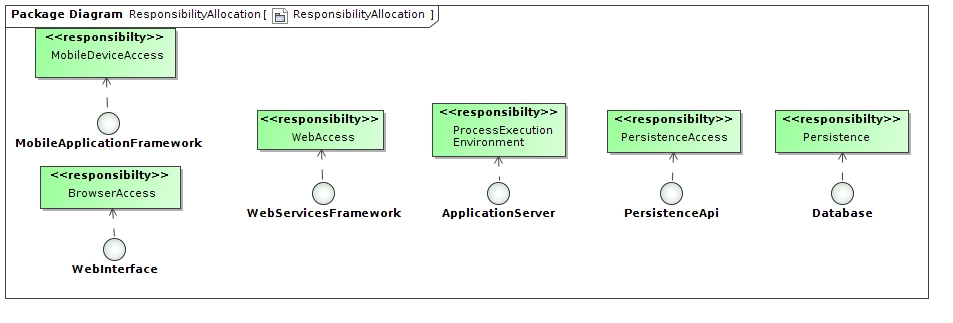
\includegraphics[width=\linewidth]{ResponsibilityAllocation.jpg}
				\caption{Responsibilities and Responsibility Allocation}
				\label{ResponsibilityAllocation}
			\end{figure}
		
		\subsection{Infrastructure}
			\paragraph\indent
			We will be using the layered system architecture. Figure \ref{LayeredAchitecture} shows the design at the first level of granularity. The layered approach with help us to develop different parts of the system concurrently with minimal dependency on other components because the layers are loosely coupled. And secondly it will control and encapsulate the complexity of the system, thus a simpler development process. Testing layers is also easier which would result in a higher quality system.
			\begin{figure}[!h]
				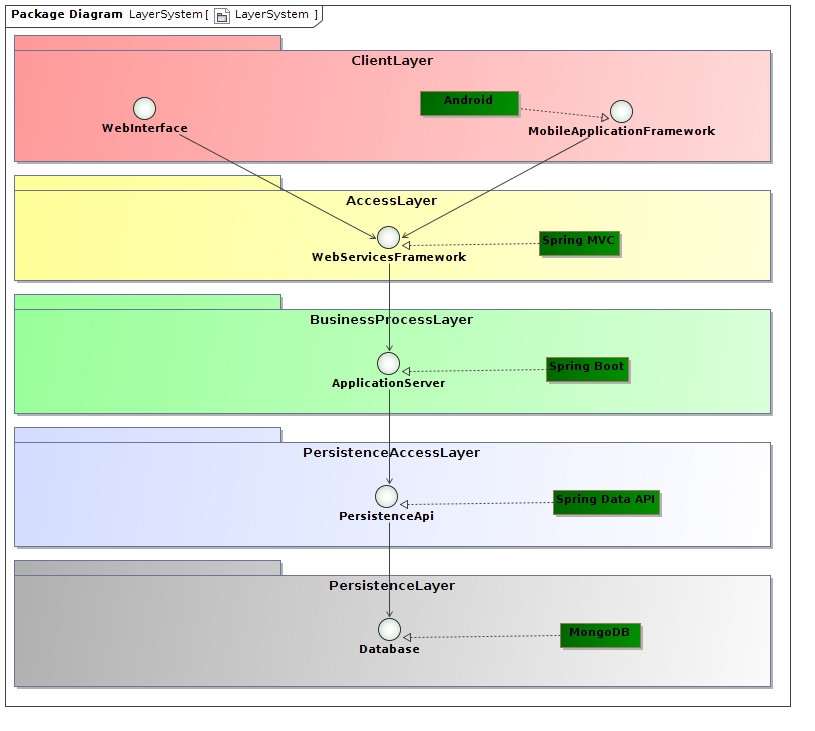
\includegraphics[width=\linewidth]{LayerSystem.jpg}
				\caption{Layered System Architecture}
				\label{LayeredAchitecture}
			\end{figure}
		
		\subsection{Tactics}
			\subsubsection{Flexibility}
				\begin{itemize}
					\item Hot deployment
					\item Contract based programming, i.e. providing proper interfaces that allows future expansion.
				\end{itemize}
			
			\subsubsection{Reliability}
				\begin{itemize}
					\item Ability to roll back database changes should an error occur during the change.
					\item Ability to restart services that have crashed due to some error that occurred.
				\end{itemize}
							
			\subsubsection{Security}
				\begin{itemize}
					\item Authentication will be required for a user to use the system.
					\item Data confidentiality will be achieved by using secure communication (HTTPS) and by applying salted hashing algorithms to keep passwords safe. Encryption will also be used on data that needs to be retrieved but has to be kept secure.
				\end{itemize}
											
			\subsubsection{Auditability}
				\paragraph\indent
				Auditability will be achieved by logging all events that occur on the server. This will ensure first of all, accountability and secondly it can assist in fault and error tracking later on.
		
	\section{Database and Persistence}
		\paragraph\indent
		We plan on using MongoDB as our database. This choice was made on the basis that a NoSQL database's graph structure would fit our application's needs better than a standard relational database. MongoDB is also the perfect tool to use when data mining and high write loads are bought into play.
	
	\section{Process Specification}
		\subsection{Server}
			\paragraph\indent
			In the back end, the system would have a polling service that polls the data sources for new information about the users. If a polling thread receives new data from the platform they add this new data to a queue to be processed. Several worker threads dequeue data from the queue and uses the natural language processing to determine the topic(s) of the data. This data is then added to a database and the corresponding topic(s) as well. Note that since hashtags are used so frequently, any hashtag in the text should be added as a topic of its own. When a user requests their bubble map, the system responds with all relevant topics of their life based on frequency and recency. These topics are then returned to the user in the form of JSON objects. Once a user expands one of the bubbles a request is sent to the server to retrieve all the relevant topic corresponding to the topic to the user. These new topic is then added to the bubble map in the form of bubbles. Relevant topics are found on the basis of your own events and the events of your friends.
		
		\subsection{Front End}
			\paragraph\indent
			The user starts out with a root bubble that has relevant topics connected to it including a friends bubble. All these bubbles can be expanded and reveal information related to that topic. The "friends" bubble shows contacts you recently communicated with or might want to communicate with now. Expanding one of these contacts will show the different platforms you can interact with this contact, including viewing a profile and sending a message/email. Other topics will expand into related topics and those can be expanded again and so forth. Upon expanding a topic a user can then interact with a specific occurrence in that topic (comment/reply) in a side panel that will be presented on the right of the screen.
	
	\section{Functional Requirements}		
		\subsection{Use Case Prioritisation}
			\textbf{Critical} (See figure \ref{UseCaseUserManagement})
			\begin{itemize}
			    \item Sign up
			    \item Choose Data Sources
			    \item Login to Data Sources
			    \item Logout
			    \item Delete Account
			\end{itemize}
			\begin{figure}[!h]
				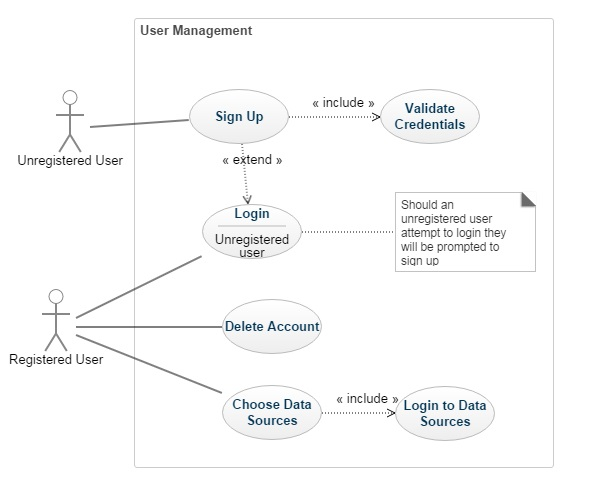
\includegraphics[width=\linewidth]{UserManagement.jpg}
				\caption{Use Case: User Management}
				\label{UseCaseUserManagement}
			\end{figure}
			\textbf{Important} (See figure \ref{UseCaseUserPreferences})
			\begin{itemize}
			    \item Expand bubble
			   	\item View bubble
			    \item Hide bubble
			    \item Minimize bubble
			\end{itemize}
			\begin{figure}[!h]
				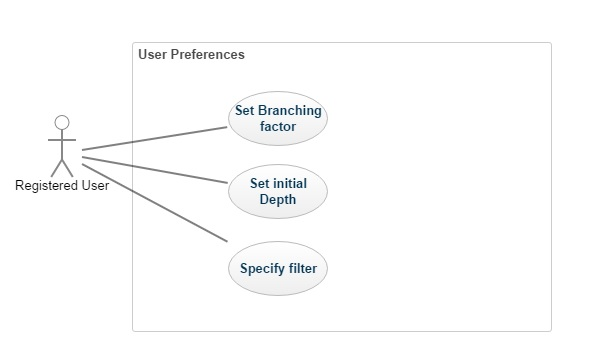
\includegraphics[width=\linewidth]{User Preferences.jpg}
				\caption{Use Case: User Preferences}
				\label{UseCaseUserPreferences}
			\end{figure}
			\textbf{Nice-to-Have} (See figure \ref{UseCaseBubbleMapInteraction})
			\begin{itemize}
			    \item Minimize bubble
			    \item Customize layout
			    \item Dedicated Android App
				\item Specify the initial depth
			    \item Specify the branch factor
			    \item Specify filter
			\end{itemize}
			\begin{figure}[!h]
				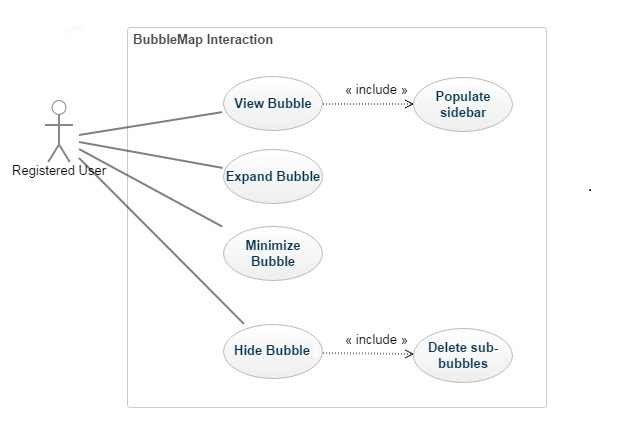
\includegraphics[width=\linewidth]{BubbleMap Interaction.jpg}
				\caption{Use Case: Bubble Map Interaction Functionality}
				\label{UseCaseBubbleMapInteraction}
			\end{figure}
		
		\subsection{Use Case/Service Contracts}
			\subsubsection{Sign up}
				\textbf{Description:}  A user is required to sign up on our system. This entails using one's Gmail account.\\
    			\textbf{Prioritisation:} Critical\\
      			\textbf{Pre-conditions}
    			\begin{itemize}
        			\item A user must have a Gmail account.
        			\item The user must enter the correct information in order for the validation to be successful.
    			\end{itemize}
    			\textbf{Post-conditions}
     			\begin{itemize}
        			\item The user will have access to the functionality provided by our system.
        			\item The user may set their preferences as they wish.
        			\item The user may add or remove data sources.
        			\item The user may log out of the system when they wish to.
        			\item The user may delete their account should they so wish.
    			\end{itemize}
    		\subsubsection{Choose Data Sources}
				\textbf{Description:}  A user is required to select the various data sources they wish to be used when extracting data to build their BubbleMap.\\
    			\textbf{Prioritisation:} Critical\\
      			\textbf{Pre-conditions}
    			\begin{itemize}
        			\item A user must be registered
        			\item A user must be logged in to the system
        			\item The user must have an active and valid account for that data source
    			\end{itemize}
    			\textbf{Post-conditions}
     			\begin{itemize}
        			\item The user may add or remove data sources.
        			\item The selected data sources will be mined for data.
        			\item The unselected data sources will not be mined for data.
    			\end{itemize}
    		\subsubsection{Login to Data sources}
				\textbf{Description:}  A user is required to provide us with their login credentials for their selected data sources.\\
    			\textbf{Prioritisation:} Critical\\
      			\textbf{Pre-conditions}
    			\begin{itemize}
        			\item A user must be logged in to the system.
        			\item A user must have selected at least one data source.
        			\item A user must have an active and valid account for that data source.
    			\end{itemize}
    			\textbf{Post-conditions}
     			\begin{itemize}
        			\item The data sources will be mined for data.
        			\item The login credentials for that data source for a specific user will be stored in our database.
    			\end{itemize}
    		\subsubsection{Logout}
				\textbf{Description:}  A user can choose to log out of the system in a secure manner.\\
    			\textbf{Prioritisation:} Critical\\
      			\textbf{Pre-conditions}
    			\begin{itemize}
        			\item A user must be registered on the system and logged in to the system.
    			\end{itemize}
    			\textbf{Post-conditions}
     			\begin{itemize}
        			\item The user will not have access to the main functionality provided by the system.
        			\item The user will need to log in again to access their BubbleMap.
    			\end{itemize}
    		\subsubsection{Delete Account}
				\textbf{Description:}  A user can choose to permanently delete their account.\\
    			\textbf{Prioritisation:} Critical\\
      			\textbf{Pre-conditions}
    			\begin{itemize}
        			\item A user must be registered on the system .
    			\end{itemize}
    			\textbf{Post-conditions}
     			\begin{itemize}
        			\item The user will not have access to the main functionality provided by the system.
        			\item The user will need to sign up again to access the system functionality.
    			\end{itemize}
		    \subsubsection{Expand Bubble}
				\textbf{Description:}  A user can choose to expand a Bubble to reveal more topics related to the Bubble.\\
			    \textbf{Prioritisation:} Important\\
      			\textbf{Pre-conditions}
			    \begin{itemize}
			        \item A user must be registered and logged in on the system.
			        \item A user must have selected data sources to be mined.
			    \end{itemize}
			    \textbf{Post-conditions}
			     \begin{itemize}
			        \item The system will expand the BubbleMap and introduce new topics.
			    \end{itemize}
			\subsubsection{View Bubble}
				\textbf{Description:}  A user can choose to view a Bubble to reveal specific data and functionality surrounding a chosen Bubble.\\
			    \textbf{Prioritisation:} Important\\
			    \textbf{Pre-conditions}
			    \begin{itemize}
			        \item A user must be registered and logged in on the system.
			        \item A user must have selected data sources to be mined.
			    \end{itemize}
				\textbf{Post-conditions}
				\begin{itemize}
					\item The system will reveal specific data regarding this topic in a side panel.
					\item The system will provide certain functionality for certain types of data e.g. a Facebook post will have the functionality to be like, commented on or shared.
				\end{itemize}
   			\subsubsection{Hide Bubble}
				\textbf{Description:}  A user can choose to hide a Bubble which will hide all Bubbles related to it.\\
			    \textbf{Prioritisation:}Important\\
     			\textbf{Pre-conditions}
				\begin{itemize}
					\item A user must be registered and logged in on the system.
					\item A user must have selected data sources to be mined.
				\end{itemize}
    			\textbf{Post-conditions}
     			\begin{itemize}
			        \item The system will hide the specified Bubble.
			        \item The system will hide all Bubbles related to the selected Bubble.
    			\end{itemize}
    		\subsubsection{Minimize Bubble}
				\textbf{Description:}  A user can choose to minimize a Bubble which will shrink the BubbleMap and essentially hide all sub-Bubbles related to it 'behind' it.\\
    			\textbf{Prioritisation:}Important\\
    			\textbf{Pre-conditions}
			    \begin{itemize}
			        \item A user must be registered and logged in on the system.
			        \item A user must have selected data sources to be mined.
			    \end{itemize}
			    \textbf{Post-conditions}
			     \begin{itemize}
			        \item The system will hide the sub-Bubbles of a selected Bubble.
			       \item The Bubble will provide the functionality to be expanded again.
			    \end{itemize}
    		\subsubsection{Specify the initial depth}
				\textbf{Description:}  A user can choose specify the extent to which the BubbleMap will bubble out i.e. the extent to which it will expand.\\
			    \textbf{Prioritisation:} Nice-to-Have\\
      			\textbf{Pre-conditions}
			    \begin{itemize}
			        \item A user must be registered and logged in on the system.
			        \item A user must have selected data sources to be mined.
			    \end{itemize}
    			\textbf{Post-conditions}
     			\begin{itemize}
        			\item The user's BubbleMap will modify itself to adapt to the user's specifications.
    			\end{itemize}
    		\subsubsection{Specify the branch factor}
				\textbf{Description:}  A user can choose specify how many branches the BubbleMap will initially have.\\
			    \textbf{Prioritisation:} Nice-to-Have\\
      			\textbf{Pre-conditions}
			    \begin{itemize}
			        \item A user must be registered and logged in on the system.
			        \item A user must have selected data sources to be mined.
			    \end{itemize}
    			\textbf{Post-conditions}
			    \begin{itemize}
			    	\item The user's BubbleMap will modify itself to adapt to the user's specifications.
    			\end{itemize}
    		\subsubsection{Specify a filter}
				\textbf{Description:}  A user can choose specify a filter to use on the BubbleMap.\\
			    \textbf{Prioritisation:} Nice-to-Have\\
    			\textbf{Pre-conditions}
			    \begin{itemize}
			        \item A user must be registered and logged in on the system.
			        \item A user must have selected data sources to Fbe mined.
			    \end{itemize}
    			\textbf{Post-conditions}
     			\begin{itemize}
        			\item The user's BubbleMap will modify itself to adapt to the user's specifications.
    			\end{itemize}
		\subsection{Required Functionality}
			Functionality that should be included in the system includes:
			\begin{itemize}
				\item A login/sign up system. 
				\item Adding various data sources to your account.
				\item Interaction with data sources directly from the mind map itself (commenting, emailing, etc.).
				\item Expanding bubbles in order to find articles related to that bubble.
				\item Rapidly integrate new information into the system.
				\item Logs will be used to track any unhandled exceptions or problems.
			\end{itemize}
			
	\section{Technologies}
		\subsection{Framework}
			\paragraph\indent
			The framework we decided to use is Spring Boot. This was chosen on the fact that Spring is a lot more lightweight than JavaEE. Spring also uses the convention-over-configuration idea that simplifies the learning experience.
			
			\paragraph\indent
			Spring is a well known framework with a large community of support. It is highly scalable and works towards being stateless. Spring also integrates well with technologies like Tomcat and build tools like Gradle. Spring Boot was chosen over Spring MVC for its simplicity.
			
			\paragraph\indent
			Research on Googles framework "Google Guice" was also done as an alternative, and while a good architecture in terms of what it does and how it makes it simpler for the programmer by moving away from XML, it is still a relatively new framework and does not have much support yet. Spring has been tried and tested and the fault tolerance on Spring is the deciding factor over Google Guice
			
		\subsection{Web Container}
			\paragraph\indent
			The web container we have chosen to use is Tomcat. Since, as mentioned before, we have chosen to use Spring as our framework Tomcat would be the obvious choice, given it good integrability with Spring.
			
			\paragraph\indent
			Jetty was also considered but due to the amount of documentation and experience that Tomcat has over Jetty, the choice was made to rather go with Tomcat. Benchmark tests were also run with Tomcat, Jetty, Glassfish and it was shown that Tomcat was the better contender.
			
			\paragraph\indent
			We have decided to move away EJB containers and thus Java EE containers to use the much lighter web container server in response to the dynamics of our particular system which required a fast, light footprint system to run our framework on.
		
		\subsection{Natural Language Processor}
			\paragraph\indent
			Google recently released their English natural language processor called Parsey McParseface. This will be used to analyse text to determine topics.
			
		\subsection{Build Tool}
			\paragraph\indent
			Gradle was chosen as the build tool due to its simplicity and simplistic integrability with Spring. It also doesn't use the XML approach that Maven uses but rather uses a more natural programming style that is recognizable.
			
		\subsection{Communication}
			\paragraph\indent
			WebSockets will be used to have a persistent client to server communication that will create a low latency, real time interaction, a requirement for our system. Some of the advantages of WebSockets is is its high scalability, high performance and protocol layering.
			
			\paragraph\indent
			A hypothesis with WebSockets initially was that not all browsers could support this technology. This was however proven incorrect as tests run with all browsers showed that every browser except Opera mini (A mobile client for Opera) supported WebSockets.\sloppy\url{http://caniuse.com/\#feat=websockets}
	
	\section{Open Issues}
		\begin{itemize}
			\item What we are going to use for our physical server?
			\item How often should the mind map refresh?
			\item How much data mining should be done before the information is displayed and the mining starts being done behind the scenes?
			\item Should removing bubbles remove data from the database or not?
			\item Is a privacy policy required?
		\end{itemize}

\end{document}
